\documentclass[10 pt]{beamer}
\usetheme{Madrid}
\usepackage[utf8]{inputenc}
\usepackage{xspace}
\usepackage{graphicx,graphics} 
\usepackage{color}
\usepackage{amsmath}
\usepackage{amsfonts}
\usepackage{amssymb}
\usepackage{amsthm}
\usepackage{algorithm}
\usepackage{algorithmic}
\usepackage{longtable}
\usepackage{complexity}
\usepackage{tkz-graph}
\usepackage{float}
\usepackage{multicol}
\usepackage{setspace}
\usepackage[absolute,overlay]{textpos}
\graphicspath{{fig/}}
\tikzset{
  LabelStyle/.style = { rectangle, rounded corners, draw,
                       font = \bfseries },
  EdgeStyle/.append style = {-} }
\title{Contention management for Deterministic Networking}

\author{Dominique Barth, {\bf Maël~Guiraud}, Brice Leclerc, Olivier Marcé, Yann Strozecki }


\institute[Nokia Bell Labs, DAVID-UVSQ] 
{
  DAVID, Universit\'e de Versailles Saint Quentin -
  Nokia Bell Labs France \\
}

\subject{Theoretical Computer Science}

\begin{document}

\begin{frame}

  \titlepage
  \centering
  
\includegraphics [width=15mm]{logod.png} \hspace{1cm} 
\includegraphics [width=20mm]{logon.png} \hspace{1cm} 
\includegraphics [width=20mm]{logo.png} \\
\end{frame}




\begin{section}{Introduction}

\begin{frame}{BTS}
  \centering
    A Base Transceiver Station
  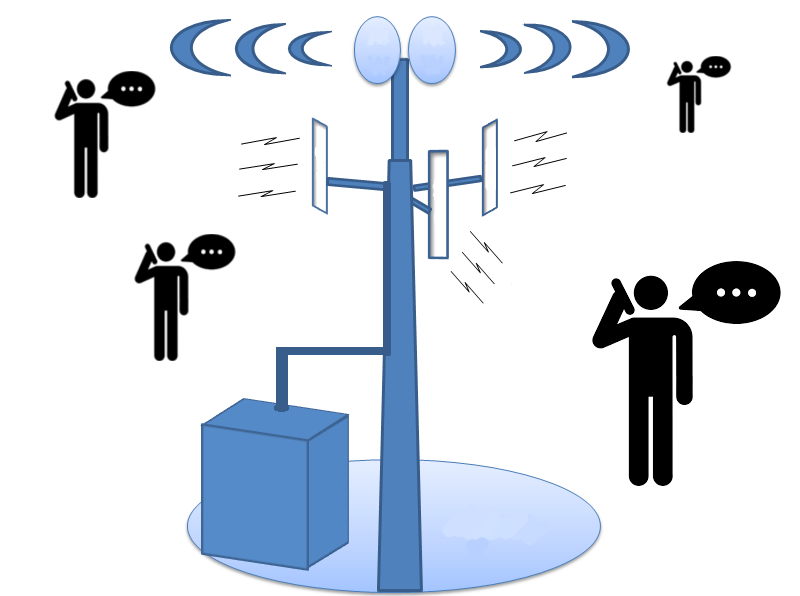
\includegraphics[scale=0.3]{btsppl.png}

\end{frame}


\begin{frame}{BBU/RRH}
  \centering
  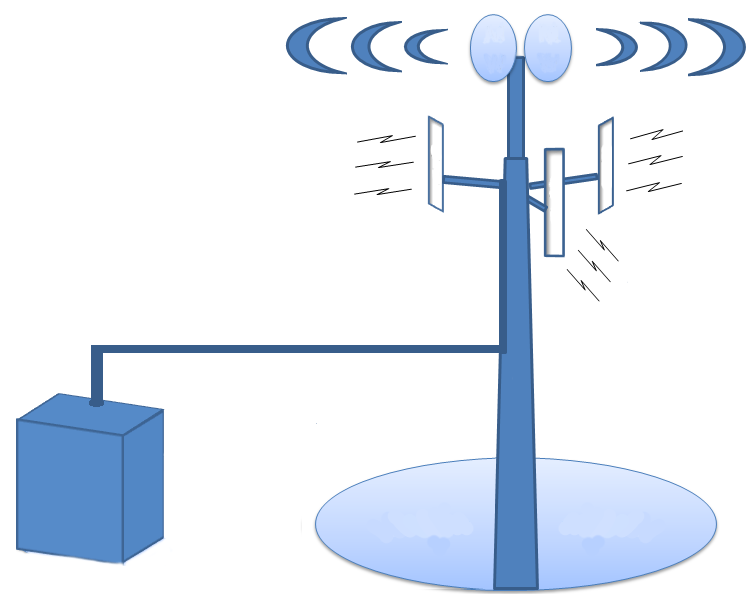
\includegraphics[scale=0.2]{cloudbts.png}\\
  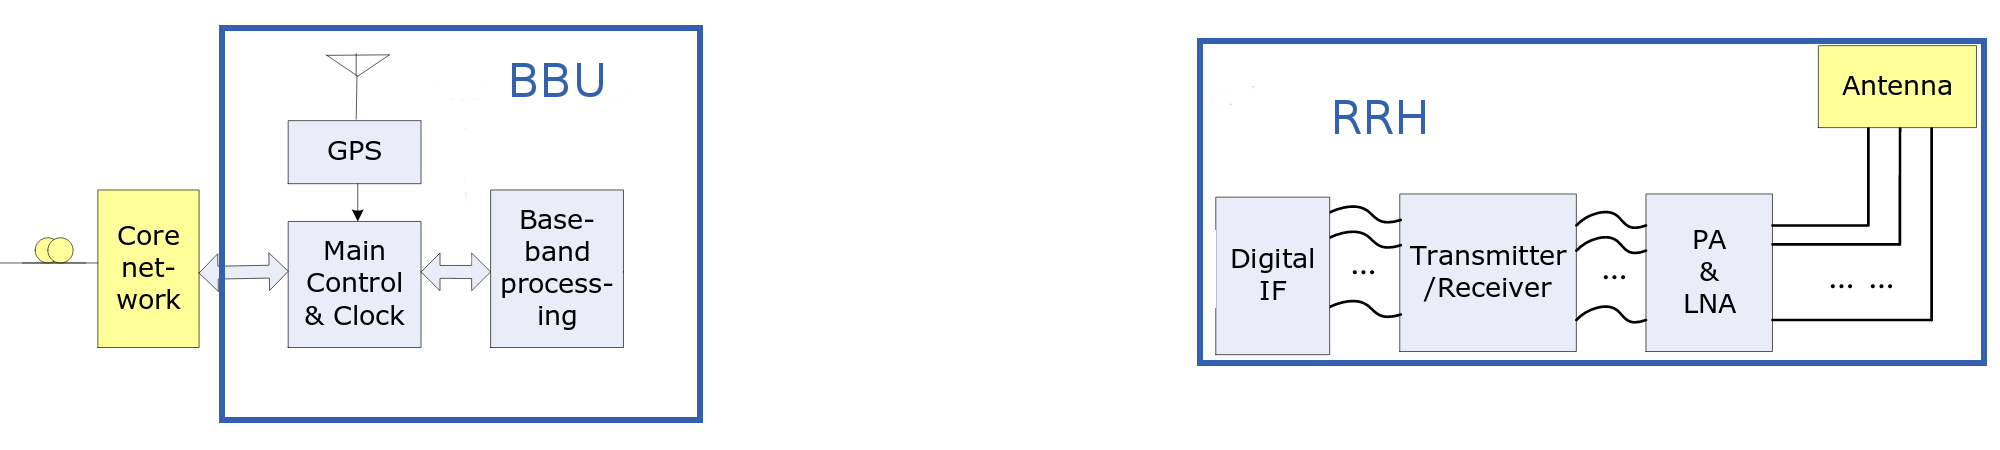
\includegraphics[scale=0.175]{BBURRH.png}
\end{frame}



\begin{frame}{Fronthaul}
  \centering
  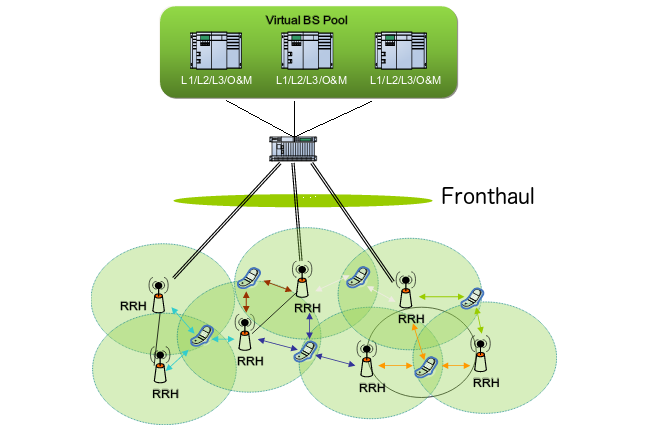
\includegraphics[scale=0.5]{CRAN}\\
  
\end{frame}

\begin{frame}{Problematic}
  \centering
  
  
 \begin{multicols}{2}
Fronthaul network 
\begin{itemize}
\item Is highly loaded
\item Periodic traffic
\item \textcolor{red}{Latency must be guaranteed}
\end{itemize}
\vspace{0.5cm}
Current approaches: \begin{itemize}
\item E2E connections $\rightarrow$ Too expensive
\item Statistical multiplexing $\rightarrow$ No latency guarantees  
\end{itemize}
\end{multicols}

\end{frame}

\end{section}

\begin{section}{Model, Problem}
\begin{frame}

  \tableofcontents[currentsection,hideothersubsections]
\end{frame}

\begin{subsection}{Network Modeling}

\begin{frame}{Model}

\centering
\scalebox{0.4}{

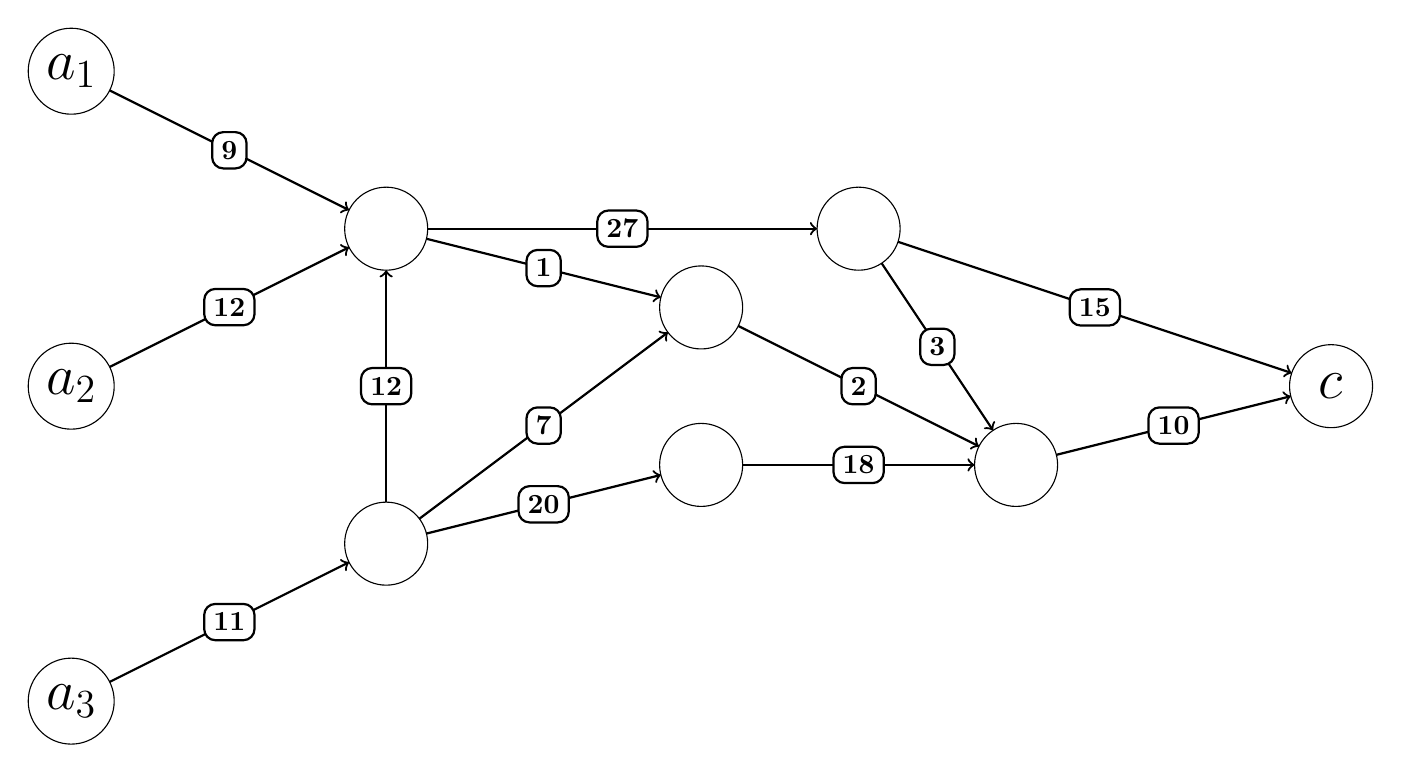
\begin{tikzpicture}
  \SetGraphUnit{5}
    \tikzset{
  EdgeStyle/.append style = {->} }
   \tikzstyle{VertexStyle}=[shape = circle, draw, minimum size = 30pt]
   \renewcommand{\VertexLightFillColor}{orange}
  \Vertex[x=0,y=0, L = {\huge $a_3$}]{a3};
  \Vertex[x=0,y=4, L = {\huge $a_2$}]{a2}
  \Vertex[x=0,y=8, L = {\huge $a_1$}]{a1}


  \Vertex[x=16,y=4, L = {\huge $c$}]{c}
  
 \SetVertexNoLabel
  \Vertex[x=4,y=2]{n1}
  \Vertex[x=4,y=6]{n2}  
  \Vertex[x=12,y=3]{n4}
  \Vertex[x=8,y=3]{n6}
  \Vertex[x=8,y=5]{n7}
  \Vertex[x=10,y=6]{n8}



  \Edge[label = 12](n1)(n2)
  \Edge[label = 3](n8)(n4)
  \Edge[label = 15](n8)(c)
  \Edge[label = 27](n2)(n8)
  \Edge[label = 7](n1)(n7)
  \Edge[label = 9](a1)(n2)   
  \Edge[label = 2](n7)(n4)
  \Edge[label = 11](a3)(n1)
  \Edge[label = 20](n1)(n6)
  \Edge[label = 18](n6)(n4)
  \Edge[label = 12](a2)(n2)
  \Edge[label = 10](n4)(c)
  \Edge[label = 1](n2)(n7)

 
\end{tikzpicture}
}
\vspace{1cm}
\begin{itemize}
\item Network : Directed Graph
\item RRH / BBU $\rightarrow$ set of vertices A (Antennas) and C (Computation)
\item  Physical Delay of a link $\rightarrow$ Weight on arcs
\end{itemize}

 \end{frame}
 
 
\begin{frame}{Routed Network}

\begin{center}
\scalebox{0.4}{

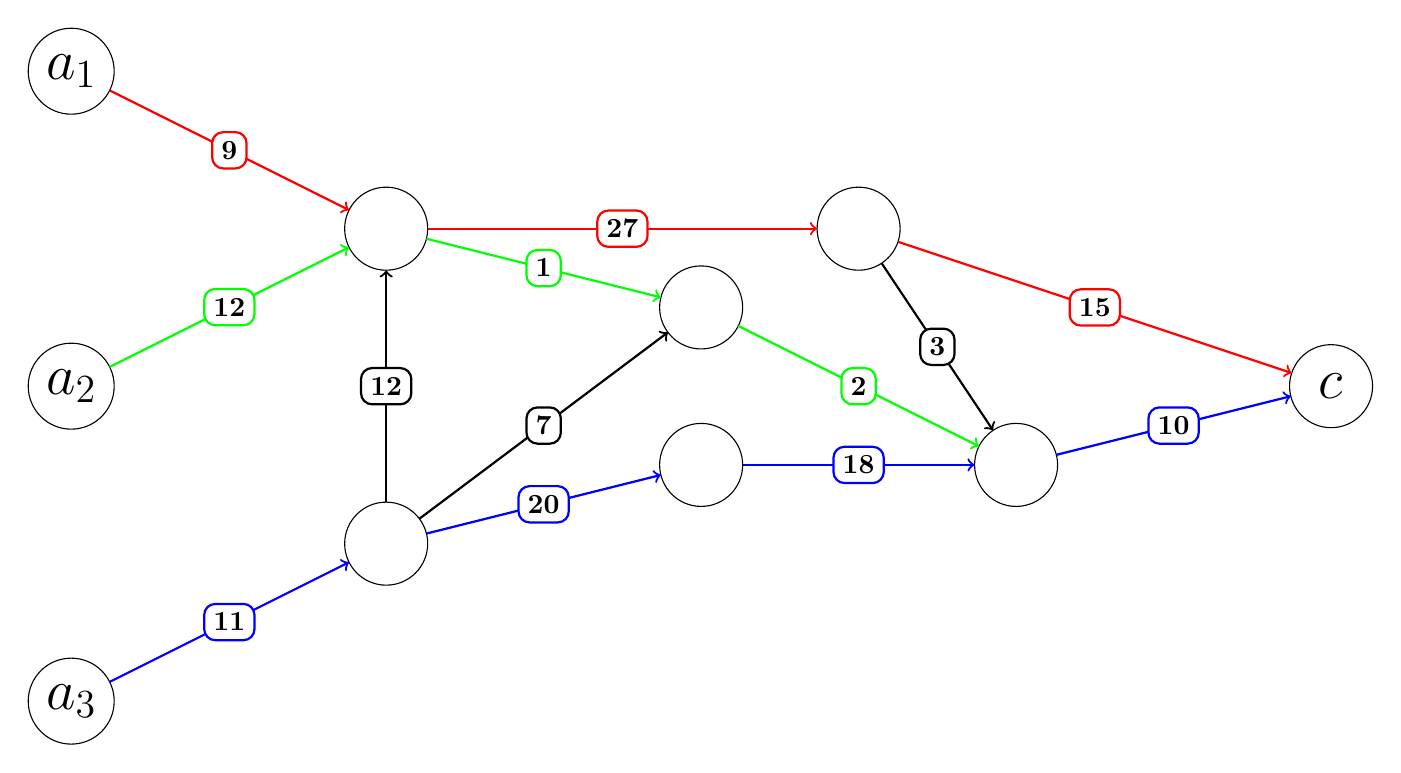
\begin{tikzpicture}
  \SetGraphUnit{5}
    \tikzset{
  EdgeStyle/.append style = {->} }
   \tikzstyle{VertexStyle}=[shape = circle, draw, minimum size = 30pt]
   \renewcommand{\VertexLightFillColor}{orange}
  \Vertex[x=0,y=0, L = {\huge $a_3$}]{a3};
  \Vertex[x=0,y=4, L = {\huge $a_2$}]{a2}
  \Vertex[x=0,y=8, L = {\huge $a_1$}]{a1}


  \Vertex[x=16,y=4, L = {\huge $c$}]{c}
  
 \SetVertexNoLabel
  \Vertex[x=4,y=2]{n1}
  \Vertex[x=4,y=6]{n2}  
  \Vertex[x=12,y=3]{n4}
  \Vertex[x=8,y=3]{n6}
  \Vertex[x=8,y=5]{n7}
  \Vertex[x=10,y=6]{n8}



  \Edge[label = 12](n1)(n2)
  \Edge[label = 3](n8)(n4)

  \Edge[label = 7](n1)(n7)

    
      \tikzset{
  EdgeStyle/.append style = {->,red} }
    \Edge[label = 9](a1)(n2)   
    \Edge[label = 15](n8)(c)
  \Edge[label = 27](n2)(n8)
  
      \tikzset{
  EdgeStyle/.append style = {->,blue} }
  \Edge[label = 11](a3)(n1)
  \Edge[label = 20](n1)(n6)
  \Edge[label = 18](n6)(n4)
  \Edge[label = 10](n4)(c) 
  
  
  
        \tikzset{
  EdgeStyle/.append style = {->,green} }
  
  
  \Edge[label = 2](n7)(n4)

  \Edge[label = 12](a2)(n2)

  \Edge[label = 1](n2)(n7)
\end{tikzpicture}
}
\vspace{1cm}
\end{center}
There is a route going from each RRH to the BBU.\\

A routed network is a graph in which the routes are given..

 \end{frame}

 
 \begin{frame}{The communication process}
Two parameters
\begin{itemize}
\item The period $P$
\item The size of a message $\tau$
\end{itemize}
\vspace{0.5cm}
The time is discretized and on each route of the network, every $P$ units of time, a message of size $\tau$ is emitted.

\vspace{0.5cm}
\begin{center}
  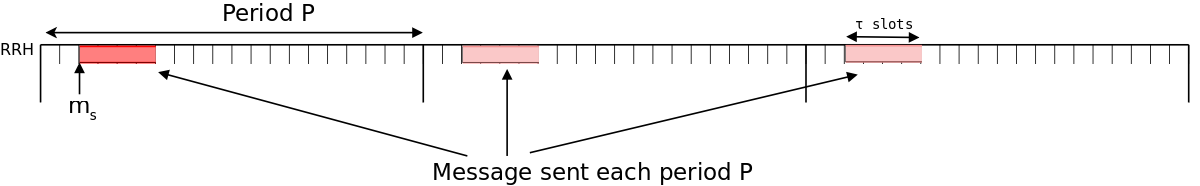
\includegraphics [width=11.5cm]{rrh} 
  \end{center}
 \vspace{0.5cm}
   
   This process is \textcolor{red}{periodic} : the message is emitted in each period at the same time, called \textcolor{blue}{offset}.
   
\end{frame}


 \begin{frame}{Collisions}

\begin{center}
\scalebox{0.4}{

\begin{tikzpicture}
  \SetGraphUnit{5}
    \tikzset{
  EdgeStyle/.append style = {->} }
   \tikzstyle{VertexStyle}=[shape = circle, draw, minimum size = 30pt]
   \renewcommand{\VertexLightFillColor}{orange}
  \Vertex[x=0,y=0, L = {\huge $a_3$}]{a3};
  \Vertex[x=0,y=4, L = {\huge $a_2$}]{a2}
  \Vertex[x=0,y=8, L = {\huge $a_1$}]{a1}


  \Vertex[x=16,y=4, L = {\huge $c$}]{c}
  
 \SetVertexNoLabel
  \Vertex[x=4,y=2]{n1}
  \Vertex[x=4,y=6]{n2}  
  \Vertex[x=12,y=3]{n4}
  \Vertex[x=8,y=3]{n6}
  \Vertex[x=8,y=5]{n7}
  \Vertex[x=10,y=6]{n8}



  \Edge(n1)(n2)
  \Edge(n8)(n4)
  \Edge(n8)(c)
  \Edge(n2)(n8)
  \Edge(n7)(n4)
  \Edge(n1)(n6)
  \Edge(n6)(n4)
  \Edge(a2)(n2)
  \Edge(n4)(c)

    
  \tikzset{
  EdgeStyle/.append style = {blue} }
  \Edge[label = 5](a1)(n2)   
   \Edge[label = 3](n2)(n7)
  
    \tikzset{
  EdgeStyle/.append style = {red} }
    \Edge[label = 2](a3)(n1)
      \Edge[label = 6](n1)(n7)
      
       \node (0) at (9,4){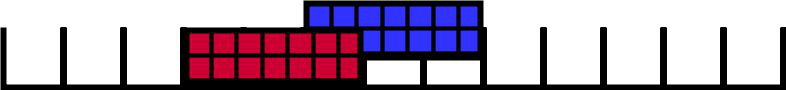
\includegraphics[scale=0.2]{col1.png}};


\end{tikzpicture}
}
\end{center}
\vspace{1cm}

There is a \textcolor{blue}{collision} between two routes when their messages go through the first vertex of a common arc at the same time.

This process is \textcolor{red}{Periodic}: everything is modulo P. 
\end{frame}

 \begin{frame}{Collisions}

\begin{center}
\scalebox{0.4}{

\begin{tikzpicture}
  \SetGraphUnit{5}
    \tikzset{
  EdgeStyle/.append style = {->} }
   \tikzstyle{VertexStyle}=[shape = circle, draw, minimum size = 30pt]
   \renewcommand{\VertexLightFillColor}{orange}
  \Vertex[x=0,y=0, L = {\huge $a_3$}]{a3};
  \Vertex[x=0,y=4, L = {\huge $a_2$}]{a2}
  \Vertex[x=0,y=8, L = {\huge $a_1$}]{a1}


  \Vertex[x=16,y=4, L = {\huge $c$}]{c}
  
 \SetVertexNoLabel
  \Vertex[x=4,y=2]{n1}
  \Vertex[x=4,y=6]{n2}  
  \Vertex[x=12,y=3]{n4}
  \Vertex[x=8,y=3]{n6}
  \Vertex[x=8,y=5]{n7}
  \Vertex[x=10,y=6]{n8}



  \Edge(n1)(n2)
  \Edge(n8)(n4)
  \Edge(n8)(c)
  \Edge(n2)(n8)
  \Edge(n7)(n4)
  \Edge(n1)(n6)
  \Edge(n6)(n4)
  \Edge(a2)(n2)
  \Edge(n4)(c)

    
  \tikzset{
  EdgeStyle/.append style = {blue} }
  \Edge[label = 5](a1)(n2)   
   \Edge[label = 3](n2)(n7)
  
    \tikzset{
  EdgeStyle/.append style = {red} }
    \Edge[label = 2](a3)(n1)
      \Edge[label = 6](n1)(n7)
      
       \node (0) at (9,4){
\includegraphics[scale=0.2]{col2.png}};


\end{tikzpicture}
}
\end{center}
\vspace{1cm}

Choosing the offset such that there is no collisions
\end{frame}
\end{subsection}




\begin{subsection}{Problem PRA}
\begin{frame}{Problem}
An \textcolor{blue}{assignment} is a choice of offsets for each route without collisions.
\vspace{1cm}

{\bf Periodic Routes Assignment (PRA)}\\
{\bf Input:} a routed network $(G,{\cal R})$, an integer $\tau$ and an integer $P$.\\
{\bf Question:} is there a $(P,\tau)$-periodic assignment of $(G,{\cal R})$ ? \\
\pause
\begin{theorem}
PRA is \NP-Hard.
\end{theorem}

\end{frame}
\end{subsection}

\begin{subsection}{\NP-Hardness}
\begin{frame}{\NP-Hardness}
\begin{center}
 
 
\scalebox{0.5}{

\begin{tikzpicture}

\tikzset{
  LabelStyle/.style = { rectangle, rounded corners, draw,
                       font = \bfseries },
  EdgeStyle/.append style = {->} }
  \SetGraphUnit{5}
  \Vertex[x=4,y=2, L =$a_3$]{s3}
  \Vertex[x=0,y=4, L =$a_2$]{s2}
  \Vertex[x=0,y=6, L =$a_1$]{s1}
  
  \Vertex[x=12,y=3, L =$c_3$]{l3}
  \Vertex[x=14,y=4, L =$c_2$]{l2}
  \Vertex[x=10,y=2, L =$c_1$]{l1}
  \tikzstyle{VertexStyle}=[shape = circle, draw, minimum size = 20pt]
     \tikzset{
  VertexStyle/.append style = {blue} }
    \Vertex[x=-8,y=3]{1}
          \tikzset{
  VertexStyle/.append style = {green} }
      \Vertex[x=-7,y=5]{2}

        \tikzset{
  VertexStyle/.append style = {red} }
      \Vertex[x=-6,y=4]{3}
             \tikzset{
  VertexStyle/.append style = {black} }
  
  
  \SetVertexNoLabel
  \Vertex[x=2,y=5]{A}
  \Vertex[x=4,y=5]{B}
  \Vertex[x=10,y=5]{C}
  \Vertex[x=12,y=5]{D}
  \Vertex[x=6,y=3]{E}
  \Vertex[x=8,y=3]{F}
  \tikzset{
  EdgeStyle/.append style = {green} }
  \Edge(s2)(A)
  \Edge(A)(B)
  \Edge(B)(C)
  \Edge(C)(D)
  \Edge(D)(l2)

  
   \tikzset{
  EdgeStyle/.append style = {red} }
  \Edge(s3)(E)
  \Edge(E)(F)
  \Edge(F)(l3) 
     \tikzset{
  EdgeStyle/.append style = {blue} }
  \Edge(s1)(A)
  \Edge(A)(B)
  \Edge(B)(E)
  \Edge(E)(F)
  \Edge(F)(l1)
  
    \tikzset{
  EdgeStyle/.append style = {black,-} }

  \Edge(1)(2)
  \Edge(1)(3)
\node (1) at (-3,4){\Huge $\rightarrow$};
\end{tikzpicture}


}\\
\vspace{2cm}
 Reducing an instance of k-coloring into an instance of our problem.
 
 \end{center}
\end{frame}
\end{subsection}

\begin{subsection}{Problem PALL}
\begin{frame}{Full process}
In each BBU, one can choose the \textcolor{blue}{waiting time} before sending back the answer.\\

\begin{center}
  \includegraphics[scale=0.7]{BBU}\\
 \end{center} 
 The \textcolor{blue}{process time} of a route is defined by $PT(r)=2\times\lambda(r)+ w_r$.\\
 
 $\lambda(r)$ is the length of the route $r$.
 
 \vspace{0.5cm}
 \pause
      {\bf Periodic Assignment for Low Latency (PALL)} 

      {\bf Input:}  A routed network $(G,{\cal R})$, the integers $P$, $\tau$ and $T_{max}$.

      {\bf Question:} does there exist a $(P,\tau)$-periodic assignment of $(G,{\cal R})$ such that for all $r \in {\cal R}$, $PT(r) \leq T_{max}$?
\end {frame}
\end{subsection}


\end{section}

\begin{section}{Results on a common topology}
\begin{frame}

  \tableofcontents[currentsection,hideothersubsections]
\end{frame}
\begin{subsection}{A star routed Network}
\begin{frame}{Star network}
  \centering
\scalebox{0.4}{
\begin{tikzpicture}
    \SetGraphUnit{5}
  \tikzstyle{VertexStyle}=[shape = circle, draw, minimum size = 50pt]
  \Vertex[x=0,y=0]{a3}
  \Vertex[x=0,y=4]{a2}
  \Vertex[x=0,y=8]{a1}
  
  \Vertex[x=16,y=0]{c3}
  \Vertex[x=16,y=4]{c2}
  \Vertex[x=16,y=8]{c1}
  
  \SetVertexNoLabel
  \Vertex[x=4,y=4]{SL}
  \Vertex[x=12,y=4]{SS}  
  \tikzset{
  EdgeStyle/.append style = {<-,green} }
  \Edge(c1)(SS)
  \Edge(SL)(a1)
  
  \tikzset{
  EdgeStyle/.append style = {blue} }
  \Edge(c2)(SS)
  \Edge(SL)(a2)
  
  \tikzset{
  EdgeStyle/.append style = {red} }
  \Edge(c3)(SS)
  \Edge(SL)(a3)
  
  \tikzset{
  EdgeStyle/.append style = {black} }
  \Edge(SS)(SL)
  


\end{tikzpicture}
}

\end{frame}
\end{subsection}

\begin{subsection}{No waiting times}


\begin{frame}{No waiting time }
The first idea is to solve PALL without waiting time in the BBU. \\

Three proposed solution :
\begin{itemize}
\item Send the message from the shortest to the longest route.
\begin{itemize}
\item The size of the period can be determined : $n\tau + 2(\lambda(r_{n-1}) - \lambda(r_{0}))$
\item Efficient for short routes but clearly bad for long routes.
\end{itemize}
\vspace{0.5cm}
\pause
\item Greedy algorithm
\begin{itemize}
\item Bound of the size of the period : $3n\tau$
\item Good complexity : $n^2$
\end{itemize}
\vspace{0.5cm}
\pause
\item Exhaustive generation
\begin{itemize}
\item Ensures to find a solution if it exists
\item FPT in the number of routes
\end{itemize}
\end{itemize}
\end{frame}


\begin{frame}{Results}
\centering
  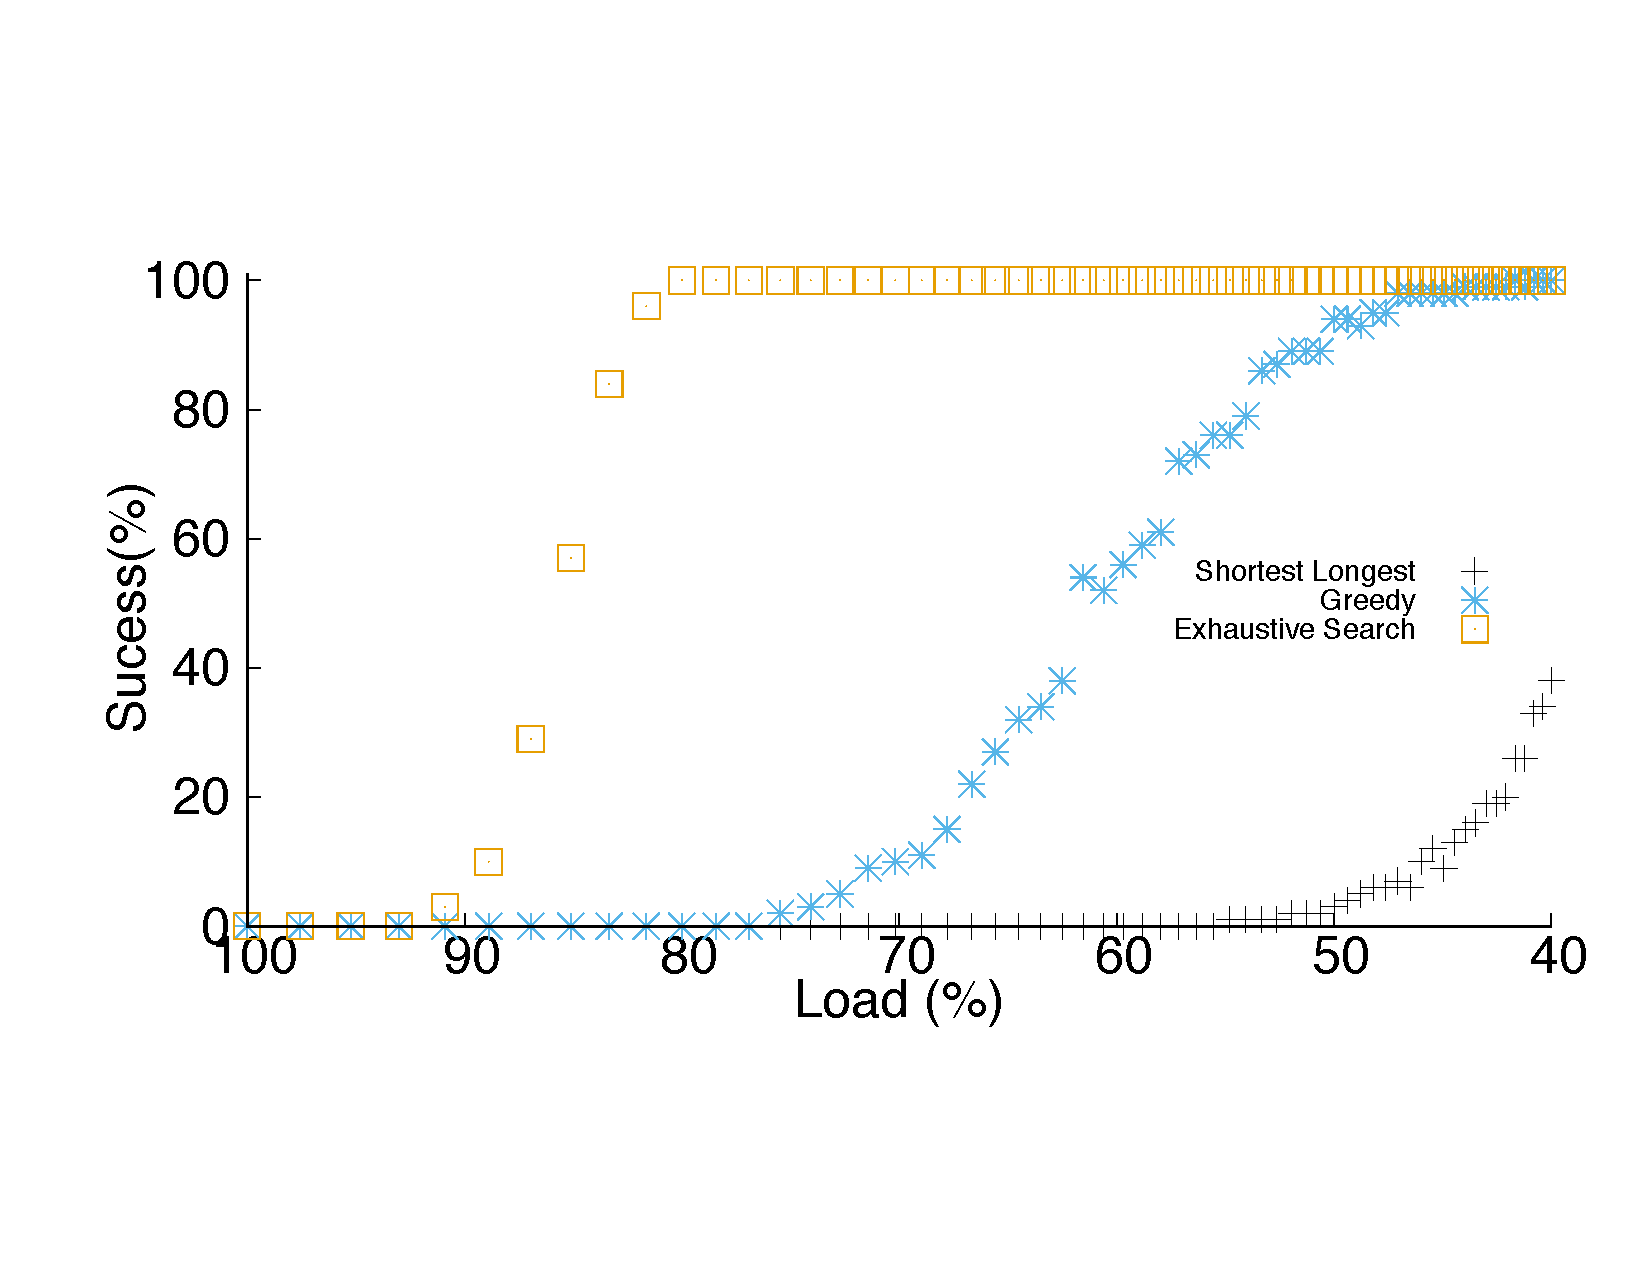
\includegraphics[scale=0.4]{echec_longues}\\
  \vspace{1cm}
  
  Not efficient under high loads : need to allow some waiting time.
\end{frame}
\end{subsection}

\begin{subsection}{Solving PALL}
\begin{frame}{A two stages approach}
To solve PALL, we first arbitrary fix the offset of the routes, then we try to solve the problem PALL in which the offset are given.

Algorithms proposed for the backward routes
\begin{itemize}
	
	 \item A greedy algorithm (GD)
	 \item Algorithm adapted for the literature (PMLS)
	 \item FPT algorithm (FPT-PMLS)
	\end{itemize}


\end{frame}
\end{subsection}

\begin{subsection}{Results}
\begin{frame}{Performances of the sending orders}
\centering
  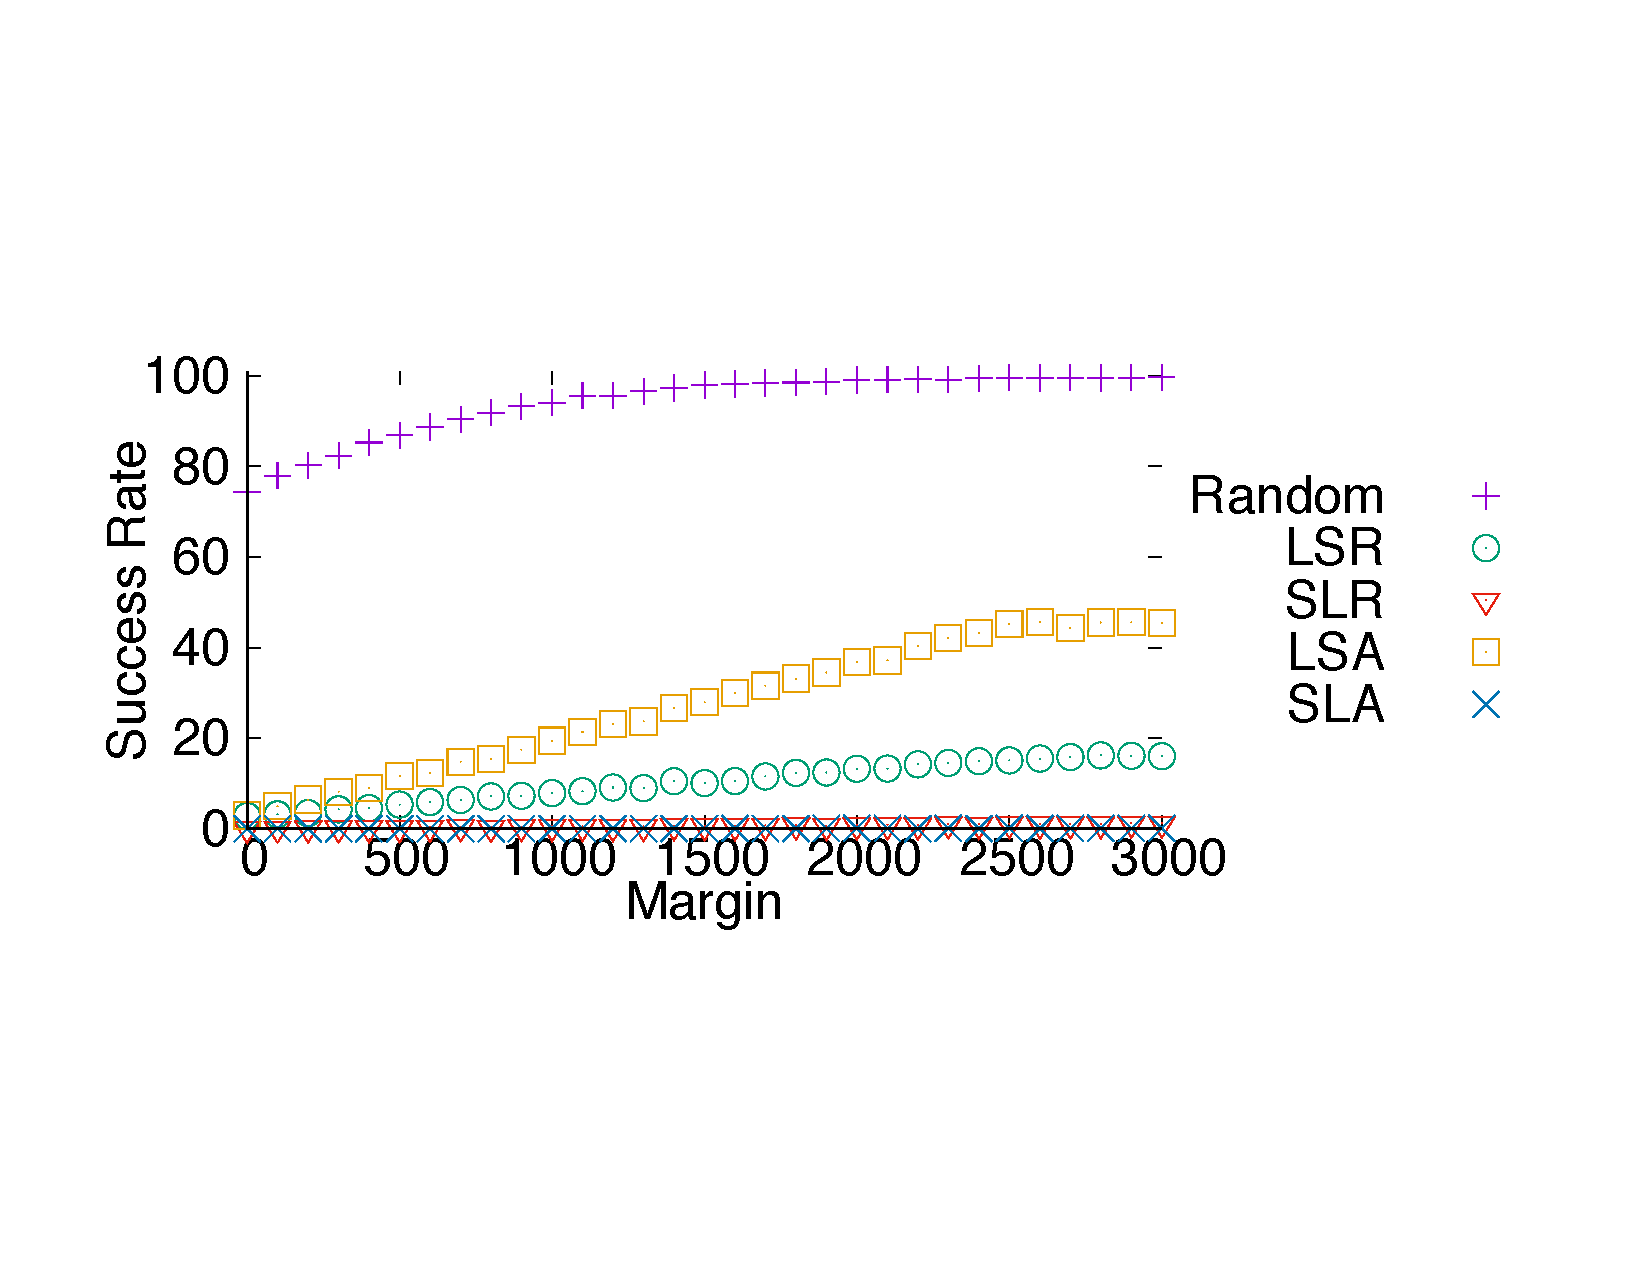
\includegraphics[scale=0.5]{departs_gp_21000.pdf}\\
  
  Random highly better, even under high loads
  \end{frame}
  \begin{frame}{Performances of the algorithms}
\centering
  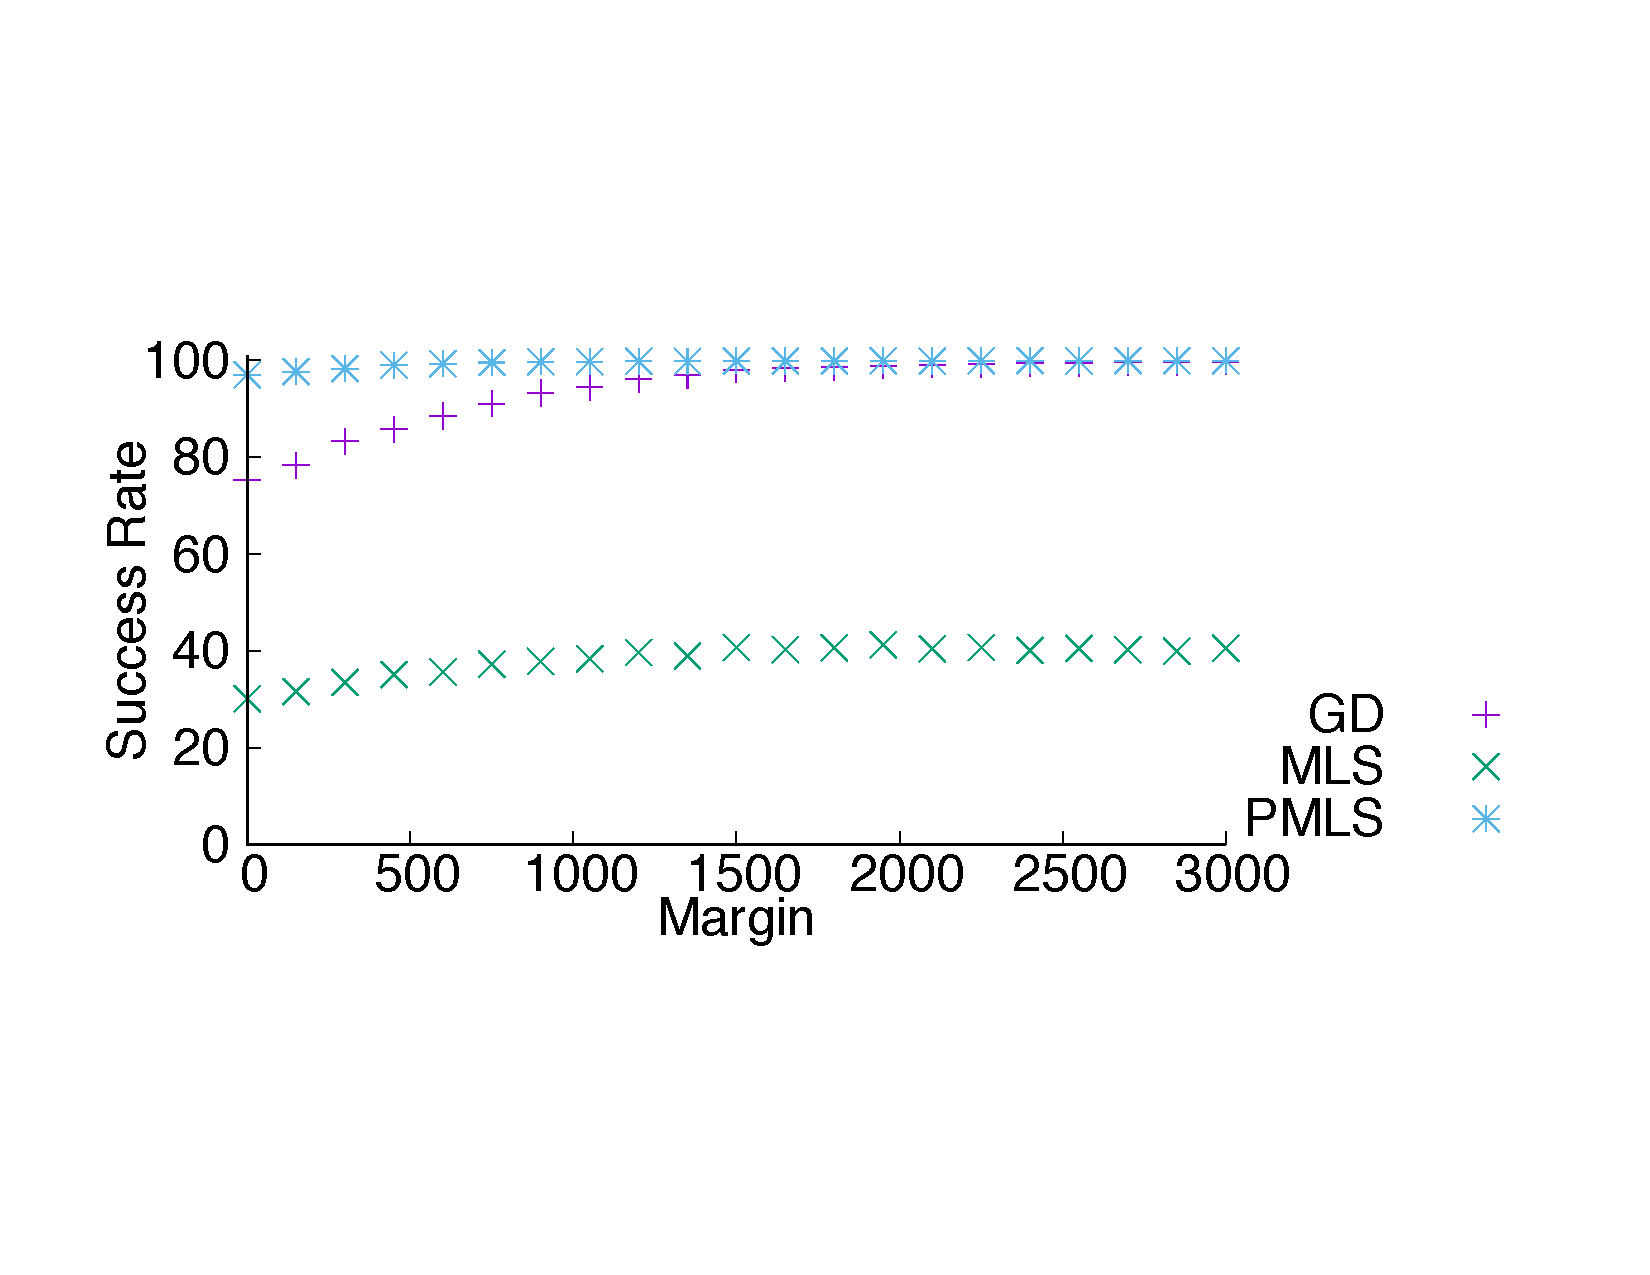
\includegraphics[scale=0.5]{retour_21000.pdf}\\
  \end{frame}
  
    \begin{frame}{Deterministic vs Stochastic}
\centering
\vspace{-2cm}
  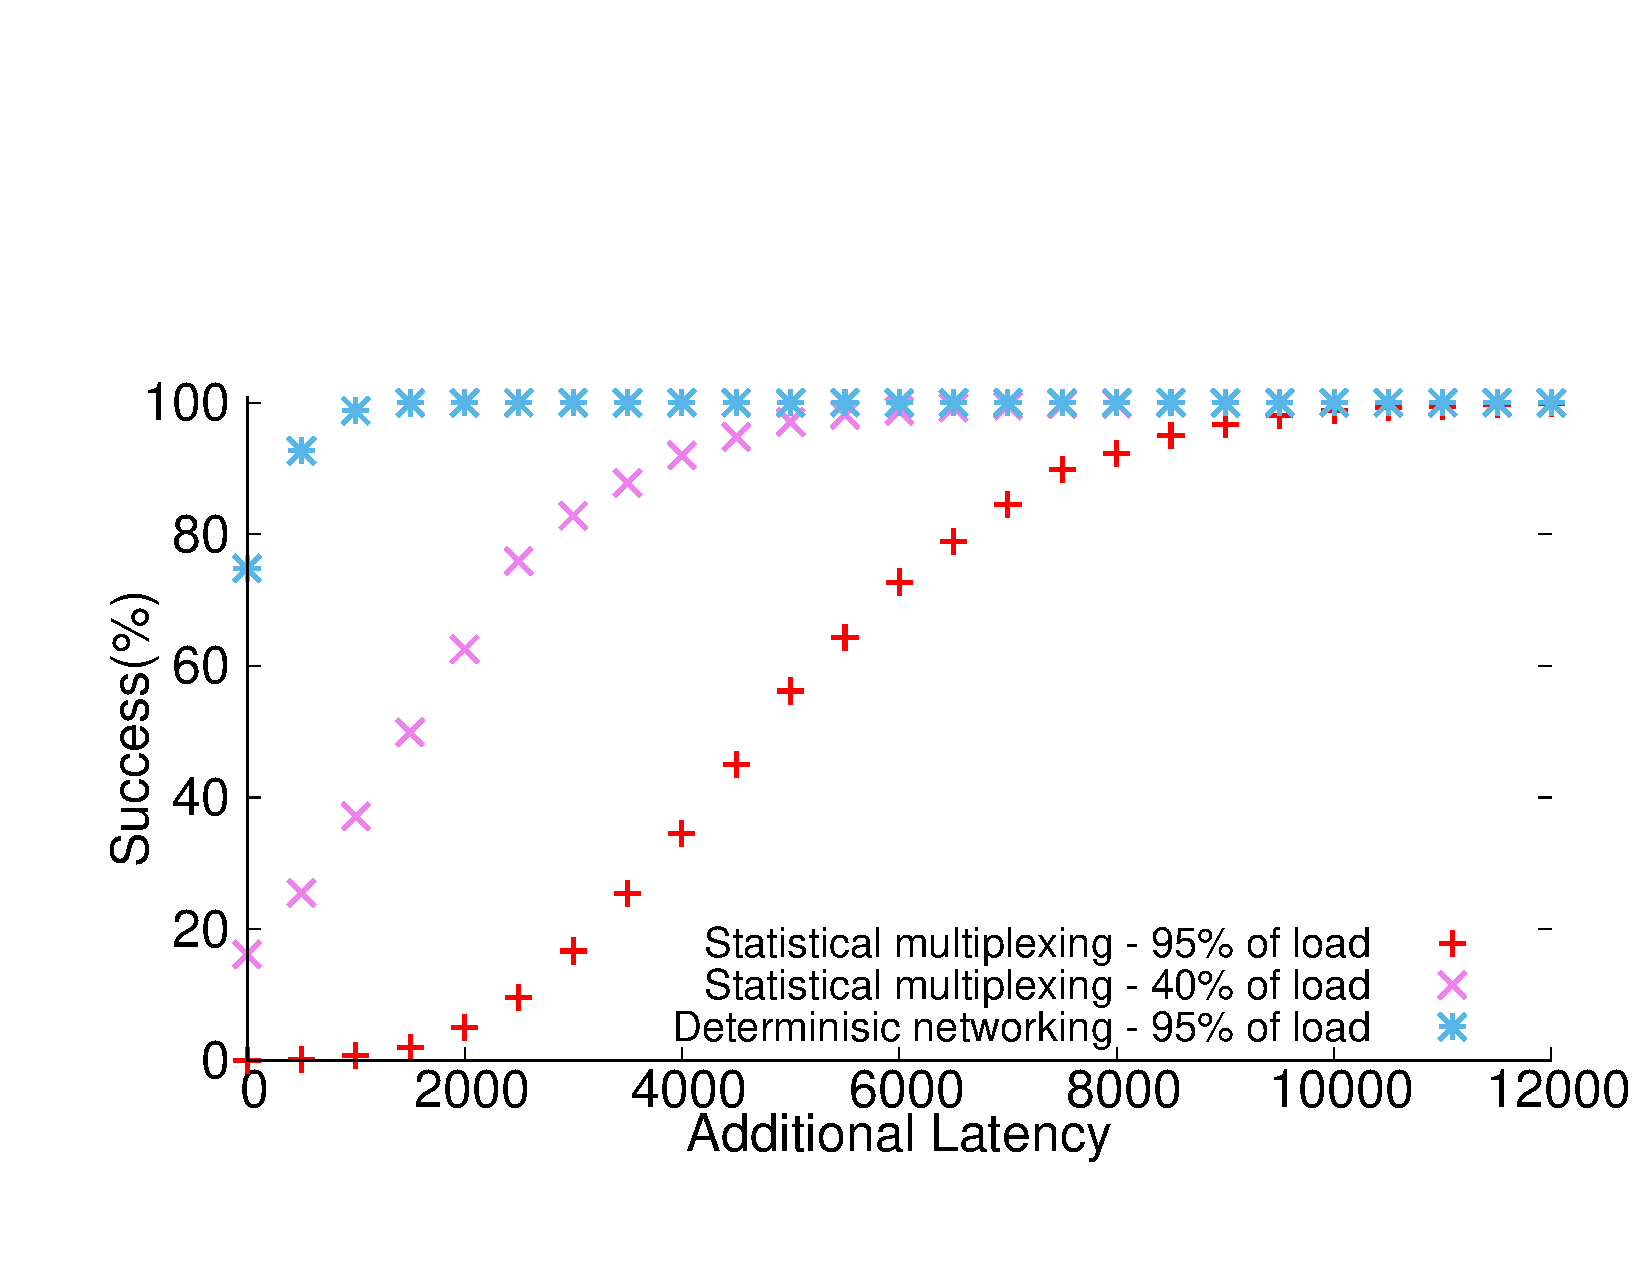
\includegraphics[scale=0.4]{stochastic.pdf}\\
  \end{frame}
\end{subsection}

\end{section}

\begin{section}{Conculsion}
\begin{frame}{Conclusion}


Perspectives :
\begin{itemize}
\item  Other topologies (trees, caterpillars, cycles, ...)
\item Choose the routes
\item Split the messages
\item Consider different kind of traffic (Best Effort, Priority)
\end{itemize}
\vspace{0.5cm}



\end{frame}

\begin{frame}
Thank you for your attention.

\end{frame}
\end{section}


\end{document}
